
%% bare_conf.tex
%% V1.3
%% 2007/01/11
%% by Michael Shell
%% See:
%% http://www.michaelshell.org/
%% for current contact information.
%%
%% This is a skeleton file demonstrating the use of IEEEtran.cls
%% (requires IEEEtran.cls version 1.7 or later) with an IEEE conference paper.
%%
%% Support sites:
%% http://www.michaelshell.org/tex/ieeetran/
%% http://www.ctan.org/tex-archive/macros/latex/contrib/IEEEtran/
%% and
%% http://www.ieee.org/

%%*************************************************************************
%% Legal Notice:
%% This code is offered as-is without any warranty either expressed or
%% implied; without even the implied warranty of MERCHANTABILITY or
%% FITNESS FOR A PARTICULAR PURPOSE! 
%% User assumes all risk.
%% In no event shall IEEE or any contributor to this code be liable for
%% any damages or losses, including, but not limited to, incidental,
%% consequential, or any other damages, resulting from the use or misuse
%% of any information contained here.
%%
%% All comments are the opinions of their respective authors and are not
%% necessarily endorsed by the IEEE.
%%
%% This work is distributed under the LaTeX Project Public License (LPPL)
%% ( http://www.latex-project.org/ ) version 1.3, and may be freely used,
%% distributed and modified. A copy of the LPPL, version 1.3, is included
%% in the base LaTeX documentation of all distributions of LaTeX released
%% 2003/12/01 or later.
%% Retain all contribution notices and credits.
%% ** Modified files should be clearly indicated as such, including  **
%% ** renaming them and changing author support contact information. **
%%
%% File list of work: IEEEtran.cls, IEEEtran_HOWTO.pdf, bare_adv.tex,
%%                    bare_conf.tex, bare_jrnl.tex, bare_jrnl_compsoc.tex
%%*************************************************************************

% *** Authors should verify (and, if needed, correct) their LaTeX system  ***
% *** with the testflow diagnostic prior to trusting their LaTeX platform ***
% *** with production work. IEEE's font choices can trigger bugs that do  ***
% *** not appear when using other class files.                            ***
% The testflow support page is at:
% http://www.michaelshell.org/tex/testflow/



% Note that the a4paper option is mainly intended so that authors in
% countries using A4 can easily print to A4 and see how their papers will
% look in print - the typesetting of the document will not typically be
% affected with changes in paper size (but the bottom and side margins will).
% Use the testflow package mentioned above to verify correct handling of
% both paper sizes by the user's LaTeX system.
%
% Also note that the "draftcls" or "draftclsnofoot", not "draft", option
% should be used if it is desired that the figures are to be displayed in
% draft mode.
%
\documentclass[conference]{IEEEtran}

\usepackage[utf8]{inputenc}
\usepackage[numbers]{natbib}
\usepackage{graphicx}
\usepackage{float}

\hyphenation{op-tical net-works semi-conduc-tor}


\begin{document}

\title{Groep 17: Impact van vergissingen bij Blackjack}

\author{\IEEEauthorblockN{Boyan Bosschem}
\IEEEauthorblockA{Hogeschool Gent\\
Bedrijf en Organisatie}
\and
\IEEEauthorblockN{Pieter- Jan Vandenberghe}
\IEEEauthorblockA{Hogeschool Gent\\
Bedrijf en Organisatie}
\and
\IEEEauthorblockN{Lorenz Verschingel}
\IEEEauthorblockA{Hogeschool Gent\\
Bedrijf en Organisatie}}

\maketitle


\begin{abstract}
Bij het gokspel blackjack zijn er technieken gekend die de spelers een voordeel geven op het casino. Toch wordt nog steeds blackjack in casino's gespeeld. Hoe komt het dat ondanks de gekende technieken het spel toch rendabel blijkt voor casino's?
\end{abstract}

\IEEEpeerreviewmaketitle

\section{Introductie}
Blackjack is een gokspel dat met speelkaarten gespeeld wordt waarbij \'e\'en of meerdere spelers tegen het huis (een dealer) spelen. Het doel van het spel is een hogere hand dan de dealer te behalen maar die niet hoger is dan 21. Het spel kent veel variaties waarbij verschillende regels van toepassing zijn. De optimale strategie\"en voor verscheidene variaties zijn reeds onderzocht en gedocumenteerd. Zo kan een speler die gebruik maakt van de beste strategie zelfs voordeel halen op het huis. Maar als dit het geval is, hoe blijft het spel dan toch rendabel voor casino's?
\\In ons onderzoek maken we gebruik van een populaire variatie van het spel en de ideale strategie voor die versie. Als doelgroep gaan we uit van de gemiddelde speler. Dit wil zeggen iemand die kennis van het spel heeft maar wel fouten kan maken. Hoeveel fouten de gemiddelde speler maakt weten we niet en dus laten we dit varie\"eren.

\subsection{De regels van het spel}

\subsubsection{Basis}
Blackjack wordt gespeeld door \'e\'en of meerdere spelers tegen het huis (een dealer). Het doel van het spel is een hogere hand dan de dealer te behalen die niet hoger is dan 21. De waarde van een hand komt overeen met de som van de waarden van alle kaarten in die hand. De waarde van elke kaart komt overeen met zijn beeltenis. Kaarten die geen getal als beeltenis hebben, hebben een waarde van tien. De aas kan als waarde zowel \'e\'en als elf aannemen. De dealer geeft elke speler twee kaarten met de beeltenis naar boven en neemt zelf twee kaarten waarvan slechts \'e\'en zichtbaar is voor de spelers. Vervolgens mag elke speler kaarten bijvragen tot men tevreden is met de hand of verloren heeft. E\'enmaal alle spelers klaar zijn is de dealer aan zet. Hij zal zijn tweede kaart tonen en altijd kaarten bij nemen tot zijn hand 17 of meer is. Indien de dealer eindigt met een hand hoger dan 21 winnen alle spelers die nog niet verloren zijn. Anders winnen alle spelers die een hogere hand dan de dealer hebben. Bij gelijkspel behoudt de speler zijn inzet. De hoogste hand is blackjack oftewel 21 met de eerste twee kaarten. Deze hand wint dus van een hand ter waarde van 21 met meer dan 2 kaarten.

\subsubsection{Verdubbelen}
Spelers krijgen vaak de mogelijkheid om hun inzet te verdubbelen wanneer hun eerste twee kaarten tesamen een waarde van negen, tien of elf hebben. Hierna krijgt de speler slechts één kaart meer. Sommige casino's laten toe om te verdubbelen ongeacht de waarde van de eerste twee kaarten.

\subsubsection{Splitsen}
Indien de eerste twee kaarten van een speler dezelfde waarde of beeltenis hebben (afhankelijk van het casino), dan mag de speler zijn hand splitsen. Hierbij speelt de speler verder met twee handen en moet dus nog eens dezelfde inzet bij de nieuwe hand inzetten. Dit mag meermaals gedaan worden zolang de gedeelde hand enkel kaarten met dezelfde waarde of beeltenis heeft. Gesplitste handen worden niet als blackjack beschouwd en hebben dus maximaal een waarde van 21.

\subsubsection{Overgeven}
Overgeven is de mogelijkheid om de helft van je inzet op te geven opdat je de andere helft mag behouden. Dit is meestal enkel mogelijk na de eerste twee kaarten

\subsubsection{Verzekeren}
Indien de zichtbare kaart van de dealer een aas is, dan heeft de speler de mogelijkheid om zich te verzekeren. Hierbij zet de speler nog eens de helft van zijn oorspronkelijke inzet in voor het geval de dealer blackjack heeft. Indien de dealer blackjack heeft, krijgt de speler evenveel terug als zijn totale inzet. Indien niet, verliest hij de verzekering en wordt het spel verder afgewerkt zoals bij normaal verloop.

\subsubsection{Zachte hand}
Ter verduidelijking vermelden we ook dat een hand die een aas bevat en dus twee waarden kan aannemen ook wel een zachte hand genoemd wordt. Dit in tegenstelling tot een harde hand die slechts \'e\'en waarde kan aannemen.

\section{Werking}
\subsection{Literatuur}
In de literatuur zijn er al ettelijke onderzoeken gedaan naar het vinden van de ideale manier om winst te maken bij het spel Blackjack.
Hieruit ontstonden strategieën, die al dan niet gebruik maken van het tellen van kaarten. \cite{thorp1961favorable} \cite{baldwin1956optimum} \cite{fogel2004evolving}

\subsection{Onderzoeksopzet}
De opzet van ons onderzoek is nagaan in hoeverre het voordeel van het huis verandert wanneer de speler meer of minder fouten maakt. We willen dus het spelgedrag van zowel ervaren spelers als spelers met beperkte kennis van het spel simuleren om daar vervolgens conclusies uit te kunnen trekken.

Zoals eerder vermeld bestaan er veel varianten van blackjack en gaan we in ons onderzoek uit van \'e\'en populaire versie. Ook maken we uitsluitend gebruik van \textit{basic strategy} \cite{thorp1961favorable}. Ervaren spelers kunnen ook aan \textit{card counting} doen oftewel kaarten tellen. Indien men kaarten telt, kan men zelfs voordeel halen op het huis \cite{fogel2004evolving}. Hoewel dit niet illegaal is, wordt dit bij casino's niet in dank afgenomen en probeert men kaartentellers buiten te houden. In ons onderzoek laten we kaarten tellen buiten beschouwing. We onderzoeken enkel het voordeel van het huis op spelers die nog niet foutloos \textit{basic strategy} kunnen spelen.

\subsection{Experiment}
Om de onderzoeksopzet te simuleren werd gebruik gemaakt van een blackjack simulator waarbij de ideale strategie en de gewenste kans op het maken van fouten kan worden ingegeven. 

Om normaal spelgedrag te simuleren werden er enkel fouten gemaakt bij grenswaarden. Men zal bijvoorbeeld nooit passen bij een hand lager dan acht of een kaart vragen bij een hand hoger dan 17. De grenswaarden kunnen terug gevonden worden in de \textit{basic strategy} tabellen bij figuren \ref{fig:normalgameplaying}, \ref{fig:doublingDown} en \ref{fig:splittingRules}. 

Elke optie die grenst aan een andere optie is een grenswaarde. Indien er een fout wordt gemaakt en er verschillende opties grenzen aan de grenswaarde, dan heeft elke optie evenveel kans op voorkomen als hoe vaak hij grenst aan de grenswaarde ten opzichte van alle andere opties. 

Neem bijvoorbeeld figuur \ref{fig:normalgameplaying}. Indien de speler een hand van zestien heeft en de dealer zijn zichtbare kaart zes is, dan is de juiste optie S oftewel passen. Indien de speler echter een fout maakt dan zal hij twee op de vijf keer zijn inzet verdubbelen (D) en drie op de vijf keer een kaart bijvragen (H) omdat deze opties in die verhouding grenzen aan de juiste optie.

Vervolgens worden voor verschillende kansen op fouten telkens 100.000 simulaties van elk 100 handen uitgevoerd. Uit de verzamelde gegevens worden het gemiddeld procentueel voordeel van het huis en de standaardafwijking berekend.

\subsubsection*{Gebruikte regels}
\paragraph{Verdubbelen}
De speler mag zijn inzet enkel verdubbelen bij de eerste twee kaarten of na een split.
\paragraph{Splitsen}
De speler mag tot maximaal vier keer splitsen zolang de waarde van elke kaart in zijn hand gelijk is.
\paragraph{Overgeven}
De speler kan zich ten alle tijde overgeven.
\paragraph{Verzekeren}
We maken geen gebruik van verzekeren in onze simulatie. Verzekeren is een optie die steeds in het nadeel van de speler is en dus best achterwege wordt gelaten. \cite{van1997blackjack}
\paragraph{Dealer}
De dealer zal altijd kaarten bijnemen tot zijn hand 17 of hoger is. Dit met uitzondering van een zachte 17 waarbij de dealer nog een kaart bijneemt.
\paragraph{Payout}
De payout is 3 : 2.
\paragraph{Inzet}
De minimale inzet bedraagt vijf eenheden. Spelers die kaarten tellen, kunnen hun voordeel vergroten door meer in te zetten wanneer de kaarten meer kans hebben om in hun voordeel te spelen. Gezien we de kaarten niet tellen, zetten we in onze simulatie steeds de minimale inzet in.


\subsection{Data}
De gevolgde strategie bij het verzamelen van de data kan gevonden worden op figuren ~\ref{fig:normalgameplaying}, ~\ref{fig:doublingDown} en ~\ref{fig:splittingRules}.

\begin{figure}[H]
	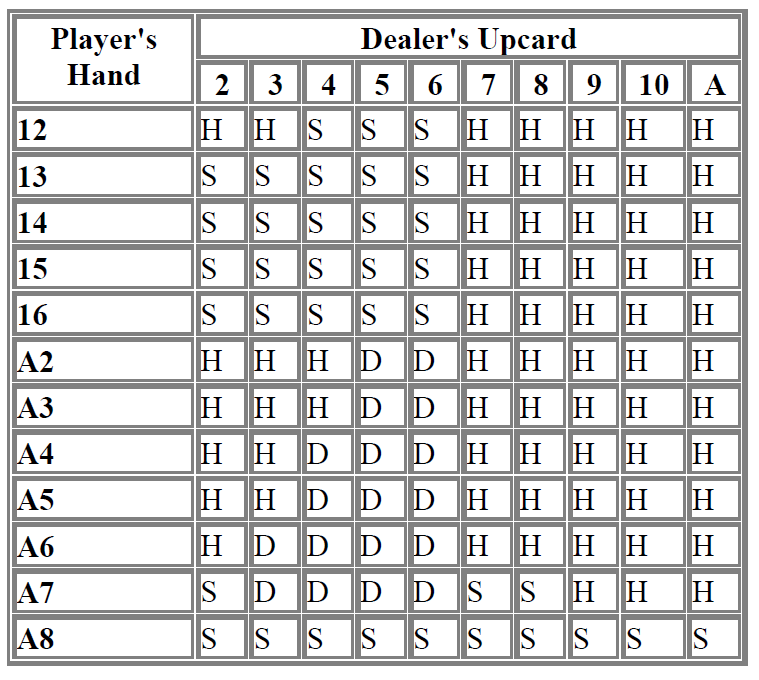
\includegraphics[width=\linewidth]{img/ThorpeNormal}
  	\caption{Normal Gameplay}
  	\label{fig:normalgameplaying}
\end{figure}
\begin{figure}[H]
	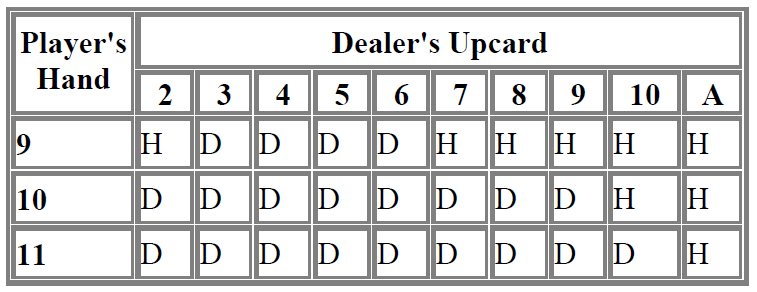
\includegraphics[width=\linewidth]{img/doubleDown}
  	\caption{Doubling down}
  	\label{fig:doublingDown}
\end{figure}
\begin{figure}[H]
	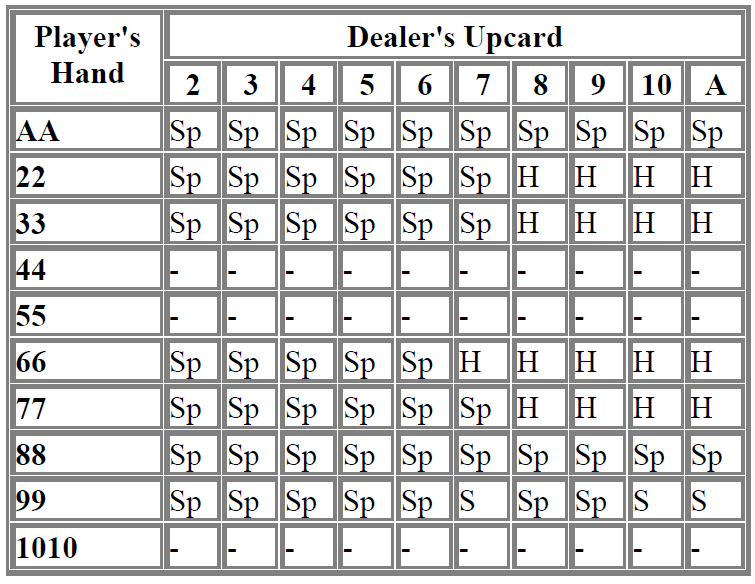
\includegraphics[width=\linewidth]{img/SplittingRules}
  	\caption{Splitting rules}
  	\label{fig:splittingRules}
\end{figure}

\begin{table}[H]
\centering
\begin{tabular}{|l|l|l|}
\hline
Kans op fout & $\mu$ & $\sigma$\\
\hline
0\% & 3,090 & 22,8915\\
1\% & 3,544 & 23,0405\\
2\% & 3,708 & 23,0394\\
3\% & 3,818 & 23,0014\\
5\% & 4,322 & 23,0957\\
7,5\% & 5,006 & 23,1455\\
10\% & 5,455 & 23,1043\\
12,5\% & 6,187 & 23,3516\\
15\% & 6,805 & 23,4473\\
17,5\% & 7,533 & 23,4688\\
20\% & 8,099 & 23,5296\\
25\% & 9,397 & 23,6362\\
30\% & 10,716 & 23,6441\\
40\% & 13,606 & 24,1438\\
50\% & 16,522 & 24,4366\\
60\% & 19,412 & 24,8674\\
70\% & 22,845 & 25,2001\\
80\% & 26,220 & 25,8522\\
90\% & 29,939 & 26,2453\\
100\% & 34,096 & 26,9239\\
\hline
\end{tabular}
\caption{Gemiddeld voordeel van het huis in functie van de kans op fouten}
\label{tab:gemiddeldesMiskansen}
\end{table}

In tabel~\ref{tab:gemiddeldesMiskansen} staat het gemiddelde voordeel van het huis in functie van de kans op fouten in het grensgebied. Deze tabel is ook uitgezet op de grafiek bij figuur ~\ref{fig:HouseEdgeMissen}. Op deze grafiek zijn ook lijnen tussen de waarden getekend ter verduidelijking, deze hebben verder geen betekenis.

\begin{figure}[H]
	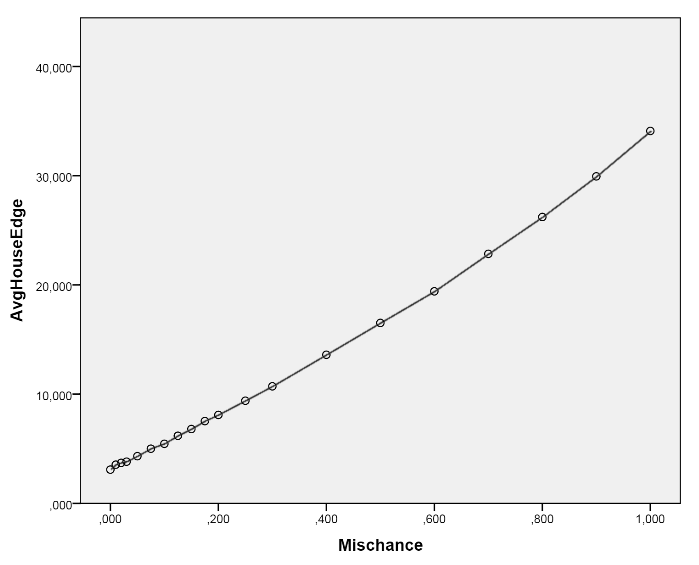
\includegraphics[width=\linewidth]{img/grafiek.jpg}
  	\caption{Grafiek: Gemiddeld voordeel van het huis (\textit{AvgHouseEdge}) in functie van de kans op fouten (\textit{Mischance})}
  	\label{fig:HouseEdgeMissen}
\end{figure}


\subsection{Analyse}
Uit de bekomen gegevens kunnen we het volgende afleiden voor de gespeelde versie van blackjack. Ten eerste blijkt dat zelfs bij foutloos \textit{basic strategy} het huis voordeel heeft op de speler. Dit lag binnen de verwachtingen \cite{fogel2004evolving}. Een speler zal dus om op lange termijn winst te kunnen maken ook moeten kunnen kaarten tellen. Ten tweede blijkt dat naarmate een speler meer fouten maakt, het voordeel van het huis lineair stijgt.

\section{Conclusie}
We concluderen dat de kans op missen in het grensgebied van de strategietabel snel een grote impact heeft op het voordeel van het huis. Het is dus voor de speler uiterst belangrijk om zo weinig mogelijk fouten te maken. Zelfs als er geen fouten worden gemaakt heeft het huis nog altijd een voordeel ten opzichte van de speler.

Hieruit kunnen we afleiden dat de meeste spelers verlies zullen maken in het casino. Enkel een kleine minderheid die foutloos blackjack speelt en kaarten telt zal op lange termijn winst kunnen maken. Deze groep wordt begrijpelijkerwijs geviseerd door casino's.

\section*{Erkenning}

Graag willen we Dhr. Van Vreckem bedanken voor nuttige tips en een duwtje in de juiste richting. Ook willen we Mvr. De Jaeger bedanken voor het kritisch nalezen en corrigeren van de paper. 

\nocite{baldwin1956optimum,bain1992introduction,kendall2003evolution}
\bibliographystyle{IEEEtran}
\bibliography{IEEEabrv,Verslag}

\end{document}


